\section{Illustrations de fonctionnalités }

	
	\subsection{Le déroulement du jeu}


		\begin{figure}
			\begin{center}
				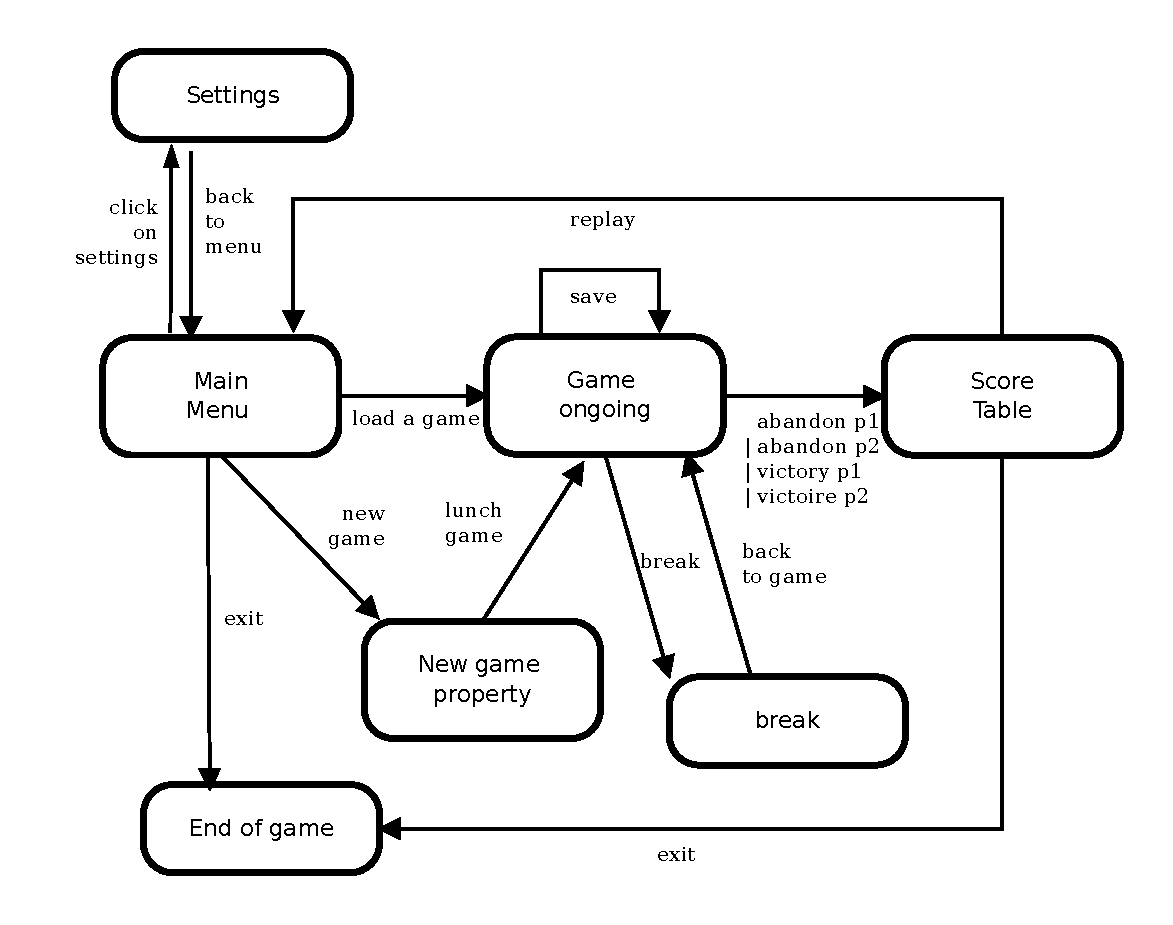
\includegraphics[width=0.7\textwidth]{figure/etat_transition_partie.pdf}
			\end{center}
			\caption{Diagrame d'états-transitions}
			\label{fig:planif}
		\end{figure}
	
		Ce diagramme d'état-transition présente les différents état dans lequel le programme \emph{Bedbihan} peut se situer, il modélise ainsi les différentes phases du jeu.


		\begin{figure}
			\begin{center}
				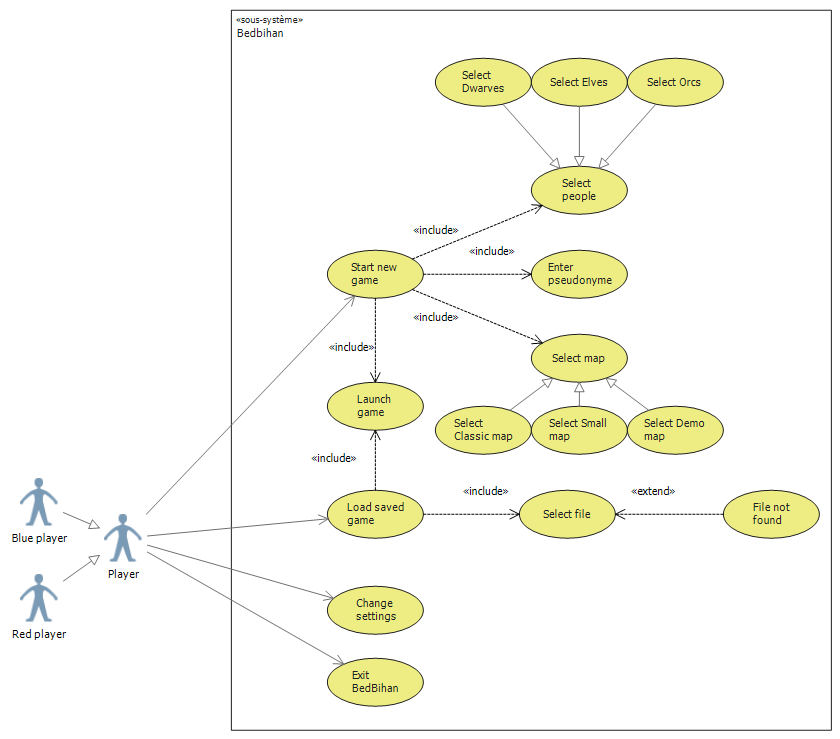
\includegraphics[width=1\textwidth]{figure/cas_utilisation_1.png}
			\end{center}
			\caption{Cas d'utilisation numéro 1}
			\label{fig:use1}
		\end{figure}

	
		Lorem ipsum dolor sit amet, consectetur adipiscing elit. Integer tempus luctus ex, non fringilla nibh laoreet non. Nullam sed enim nec leo dapibus tincidunt. Nulla augue est, cursus tempus tristique eget, venenatis sed leo. Nam eget purus lacinia, porttitor dolor eu, consectetur turpis. Suspendisse sed viverra tellus. Aliquam malesuada sed magna mattis dapibus. Pellentesque eu molestie ligula. Pellentesque dictum ultricies sagittis. Ut semper, est vitae malesuada facilisis, magna velit laoreet lectus, semper suscipit sapien lacus sed nulla.

		Aliquam finibus est ac cursus cursus. Fusce in libero ut nisi laoreet sodales. Cras vestibulum nec nulla in consequat. In eget lacus ut ipsum placerat ultrices. Nam diam magna, fermentum aliquam libero at, ornare eleifend diam. Sed et mi eget arcu bibendum congue. Vivamus in enim mollis, blandit sem in, hendrerit tellus.


	\subsection{ le déroulement d'un tour }
		\begin{figure}
			\begin{center}
				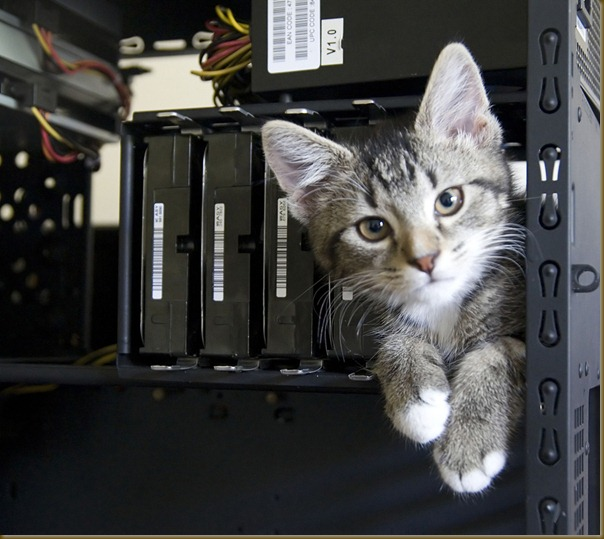
\includegraphics[width=1\textwidth]{figure/cas_utilisation_2.jpg}
			\end{center}
			\caption{Cas d'utilisation numéro 2}
			\label{fig:use2}
		\end{figure}

		Mauris rhoncus tempor rhoncus. Vestibulum lacinia tincidunt sem ac auctor. Maecenas a lectus in nisi aliquet feugiat. Sed gravida laoreet maximus. Donec feugiat vestibulum neque sit amet mollis. Maecenas commodo luctus augue et molestie. Maecenas viverra semper massa, blandit commodo lacus blandit a. Proin sed euismod massa. Aenean nec nisl sed nisi mollis congue quis a nisi. Pellentesque habitant morbi tristique senectus et netus et malesuada fames ac turpis egestas. Suspendisse tincidunt euismod ipsum vitae commodo. Ut dapibus tellus nec libero egestas, eu venenatis dolor fermentum. Donec porttitor erat ante, at tincidunt lacus efficitur vitae.

